\subsection{Context}
	The suspension on a mountain bike plays a vital part in the rider's performance, comfort and overall enjoyment of the sport. With some suspension units costing upwards of \pounds1000 it is vital that they are setup to function correctly. The objective of this thesis is to research the characteristics of mountain bike suspension, look at methods and applications of image analysis, and produce a prototype mobile application which utilises image analysis to aid the user in setting up their suspension.
\subsection{Background}
	A survey carried out by the International Mountain Bike Association shows the average price of mountain bikes owned in Europe to be \euro2546 (\pounds2206) \citep{imbasurv}. Starting at approximately \pounds1000 \citep{giantstance}, enthusiast level mountain bikes can be purchased with suspension for both the front and rear wheels, known as \gls{fs} bikes whereas \gls{ht} bikes have only front suspension; this difference can be seen in figure \ref{fig:fsandht}. Even at this comparably low cost, the suspension units have multiple adjustments available to optimize and personalize how they operate.
	\begin{figure}[h!]
		\centering
		\begin{minipage}{0.45\textwidth}
			\centering
			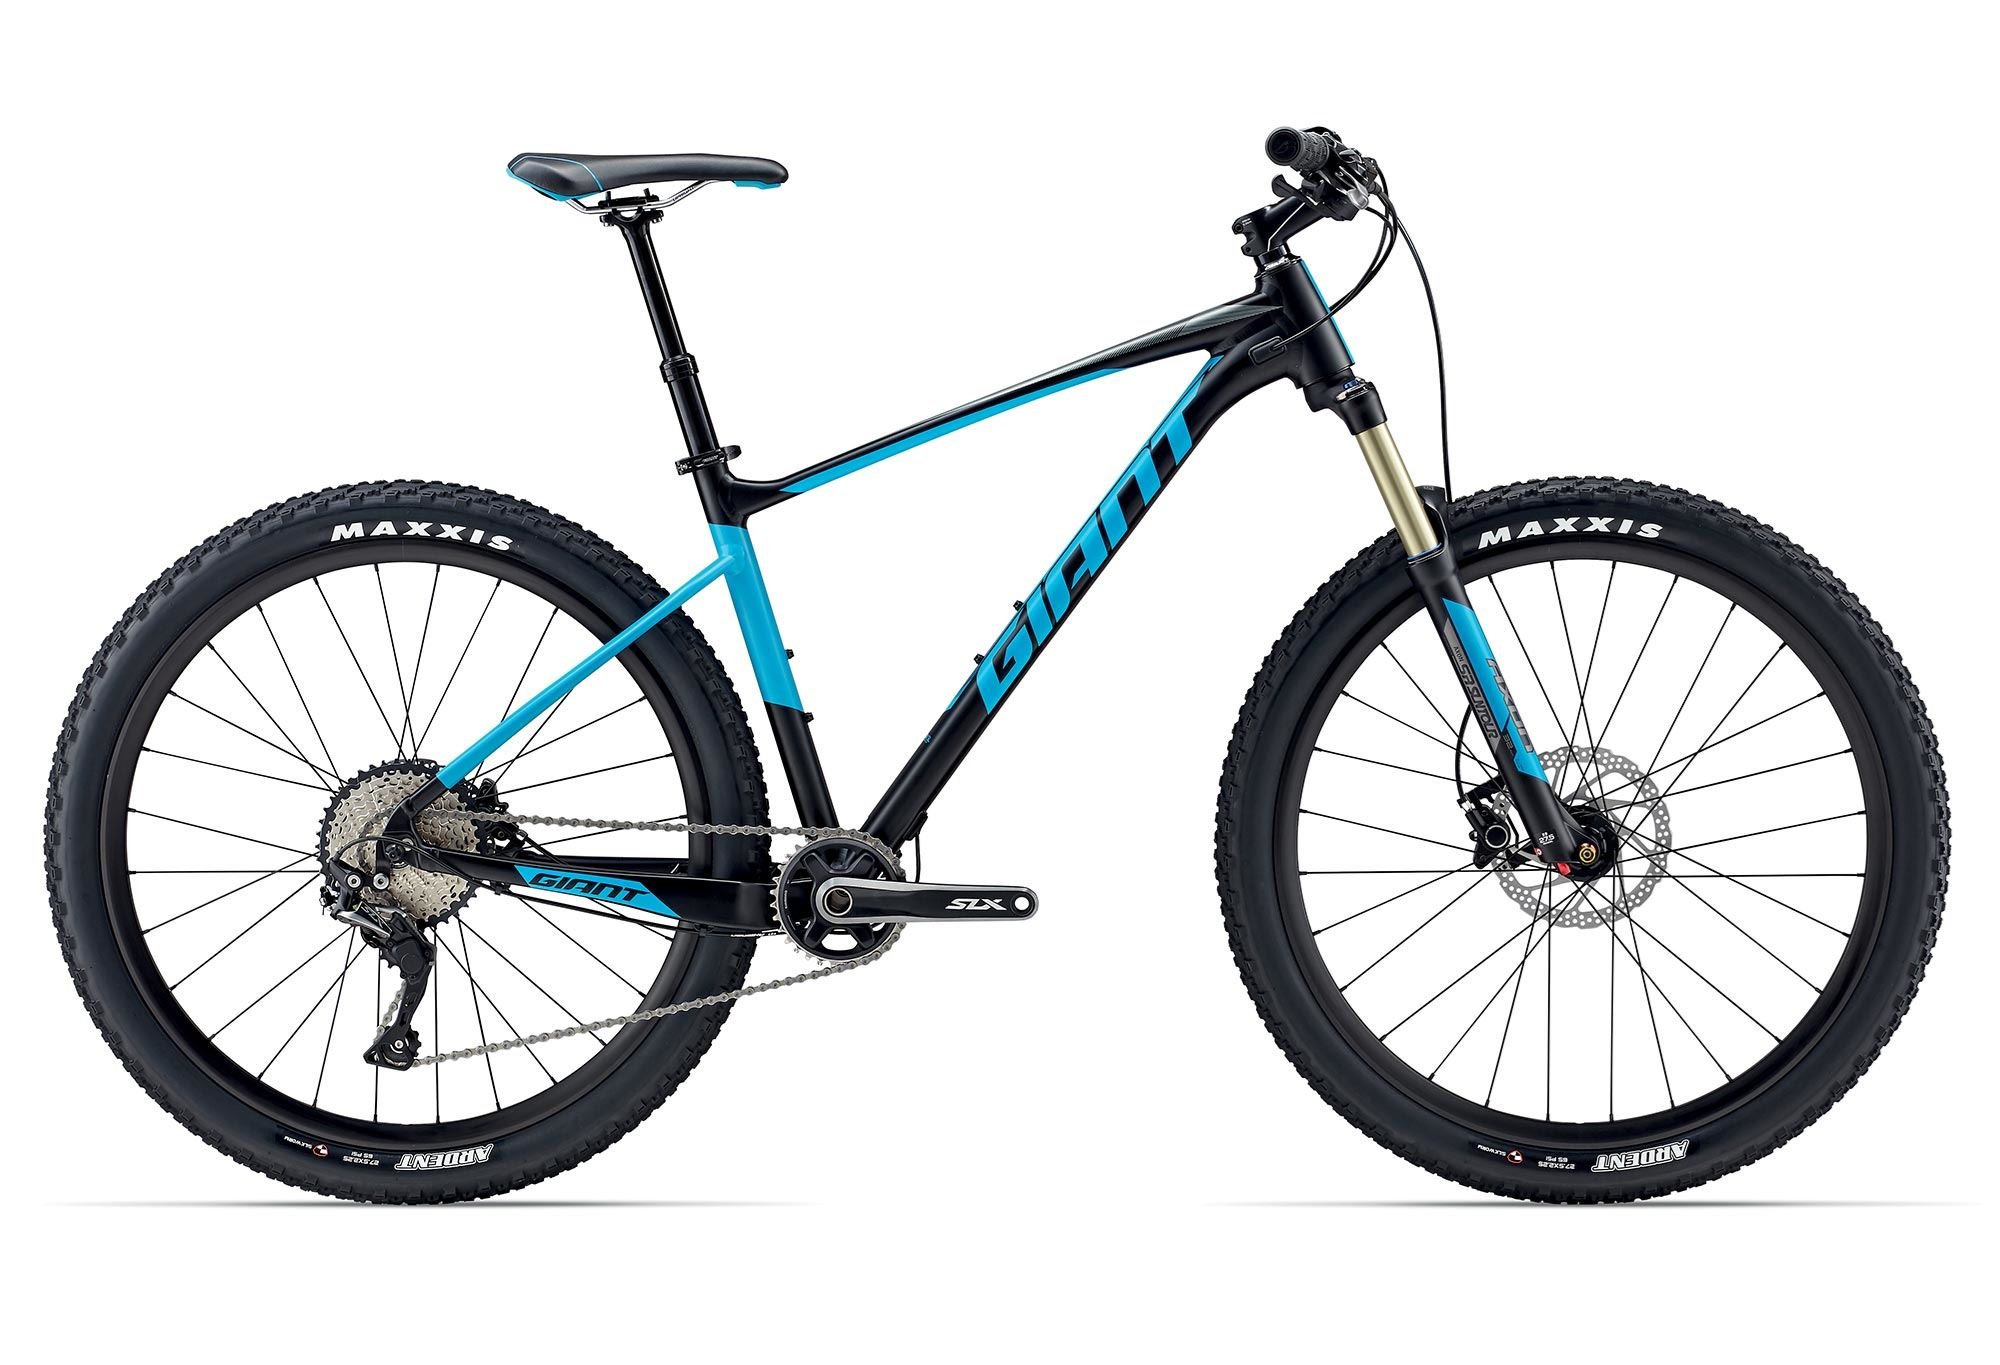
\includegraphics[width=8cm]{../images/2017_GIANT_FATHOM_1.jpg}
		\end{minipage}\hfill
		\begin{minipage}{0.45\textwidth}
			\centering
			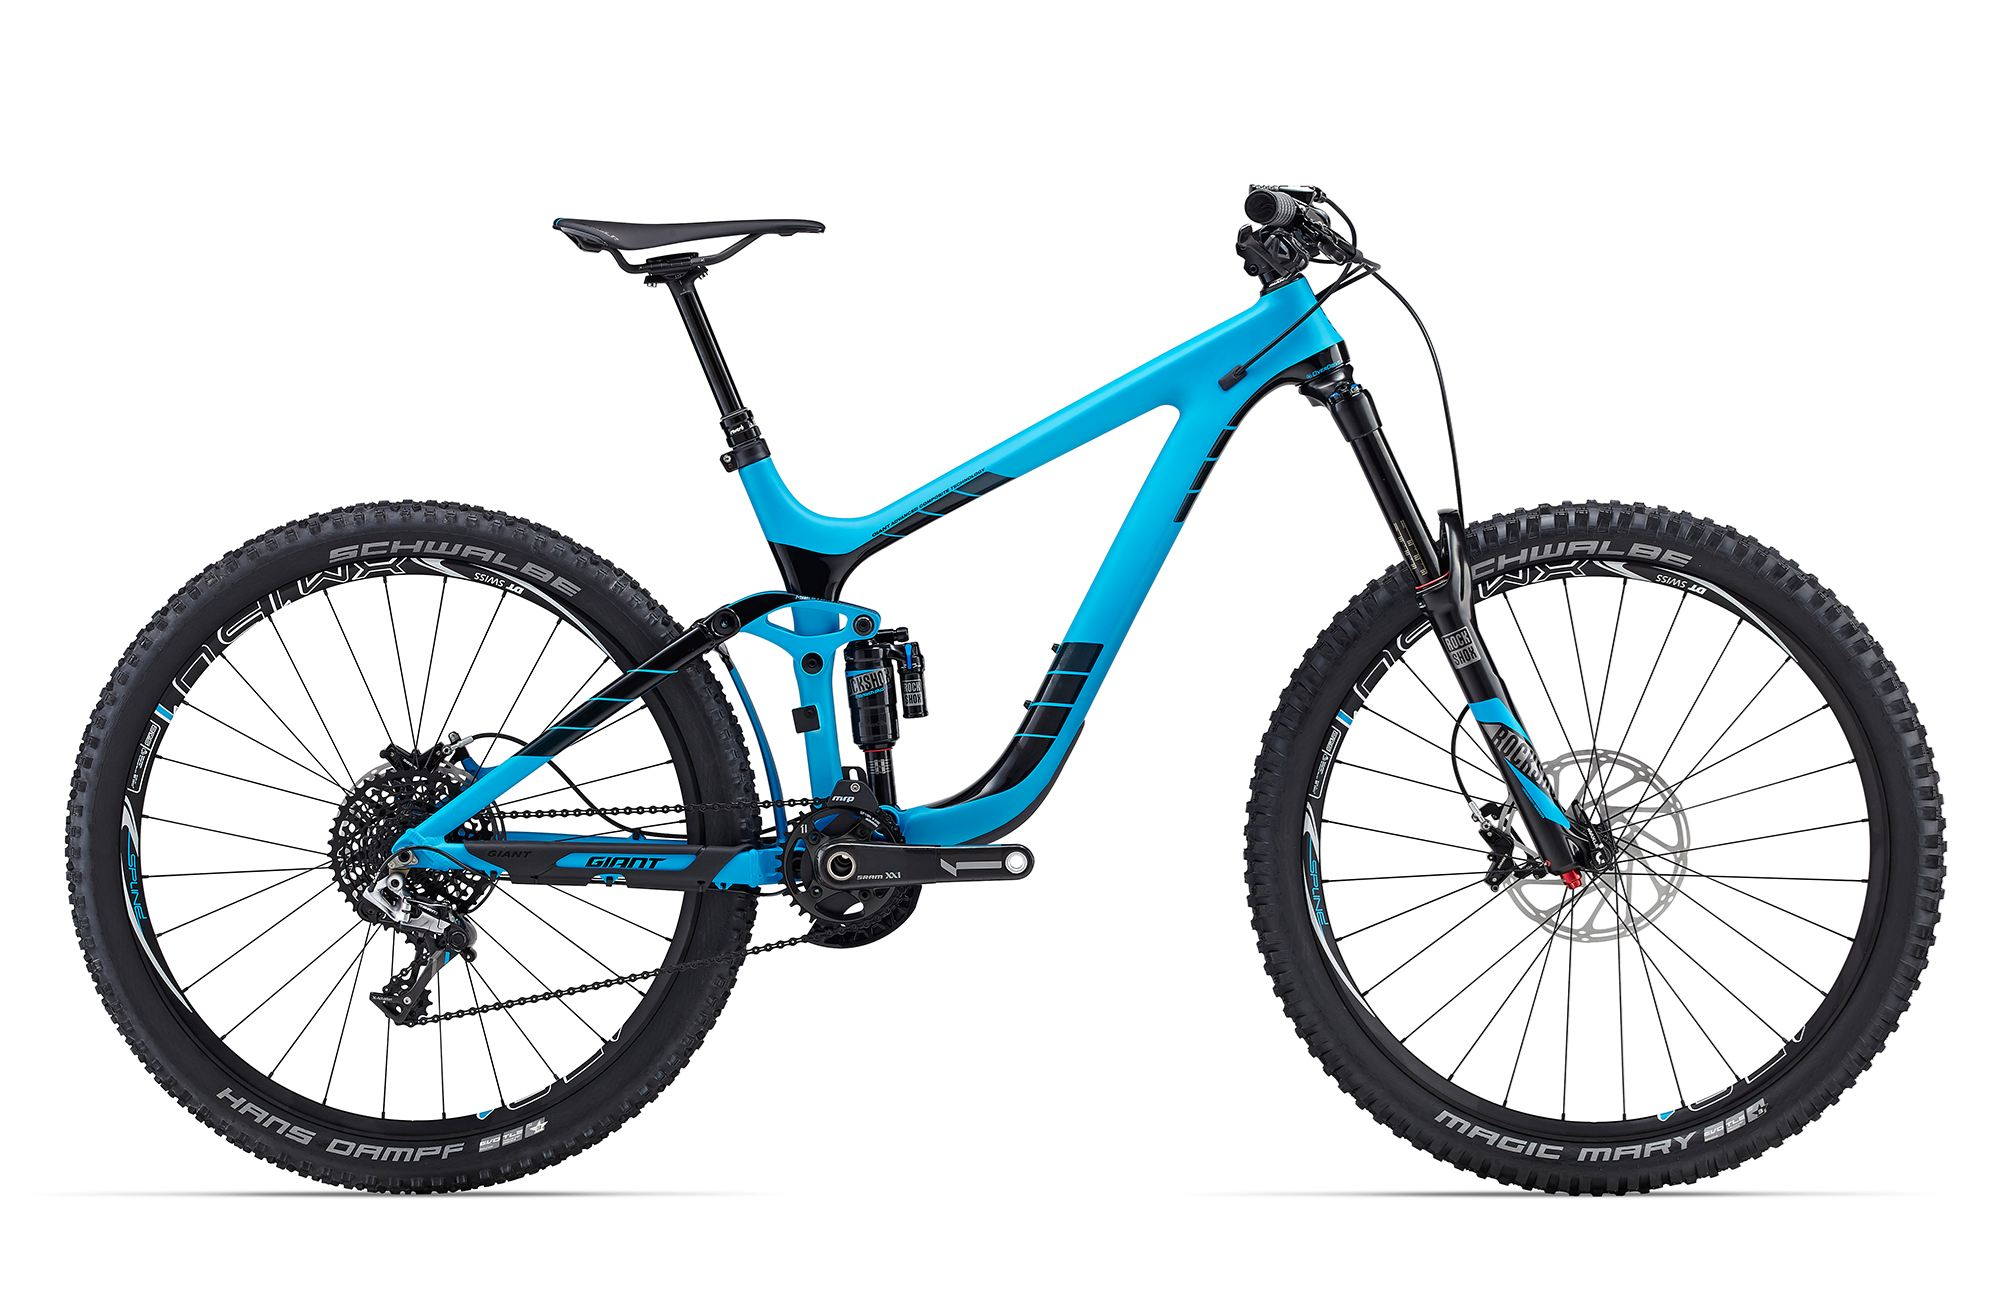
\includegraphics[width=8cm]{../images/2016_Giant_Reign_Advanced_275_0.jpg}
		\end{minipage}
		\caption{Full suspension and hardtail mountain bikes \citep{giantfathom,giantreign}}
		\label{fig:fsandht}
	\end{figure}
	\\
	To ensure the \gls{fork} and \gls{shock} function correctly they must be set up for the rider's weight and intended use of the bike. As this is considered a specialist area, many entry and mid level riders will lack the knowledge of this process or be unsure of how the suspension should operate meaning the rider could use the bike without the suspension set up correctly.
	\\\\
	It has been proven that using a \gls{fs} over a \gls{ht} offers a performance advantage to the rider \citep{fullsusperf}. However if the suspension fork and/or shock have not been set up, it can be detrimental to the rider's performance and potentially lead to injury. For example, if a shock has too little \gls{rebounddamping} set and the rider goes off a jump, the excessive speed at which the rear of the bike extends can create forwards rotation, causing the rider to go over the handlebars of the bike.
	\\\\
	Additionally, an incorrect suspension setup can cause excessive wear and tear on the bike's frame and components. Suspension which is set too soft can allow for bottoming out which expends excess forces into the frame and potentially cracks the frame's structure. Suspension set too hard forces energy, which it would normally soak up, into the wheels and tires causing denting and warping of the wheel rims. Further effects of suspension setup will be explained in following sections.
	\\\\
	Many bicycle retailers will set up the suspension on a newly purchased mountain bike for the customer on delivery. Most of the time this will be enough to avoid incident but due to the extra weight of the equipment riders use, i.e. helmet, hydration pack, body armor which the customer will not be wearing at the time of delivery, this setup is regularly inaccurate. Furthermore, with some manufacturers choosing direct sales over local retailers \citep{roseonline, ytonline}, this setup can be circumnavigated altogether.
	\\\\
	Since the birth of the modern smartphone in 2007 brought along by the first generation Apple\textregistered\ iPhone\textregistered\ and introduction of the Android\texttrademark\ mobile operating system, the use of mobile computing in everyday life has grown rapidly. Google\texttrademark\ stated that there were approximately 1.4 active Android users worldwide in 2015 \citep{androidusers}.
	\\\\
	The introduction of activity tracking devices and mobile applications such as FitBit \citep{fitbit} and Strava \citep{strava} and their growing popularity \citep{apppopularity} shows that individuals are welcome to the idea of using smartphones to aid or augment their participation in hobbies or sports. Due to this popularity and in a bid to give every rider the ability to setup and tune their own suspension, either at home or while out on a ride, companies have set about producing small devices \citep{sussmybike, shockwiztrademark} and mobile applications \citep{foxird} which aid riders in the process.
\subsection{Aims and Objectives}
	The aim of this project is to create a prototype mobile application for the Android operating system capable of providing the user with a suggested suspension setup using image analysis techniques. This will be achieved by meeting the following objectives:
	\begin{itemize}
		\item Complete a literature review of mountain bike suspension and image analysis techniques.
		\item Investigate current applications and products with similar aims
		\item Design the prototype application
		\item Implement the prototype application 
		\item Evaluate the produced application against current products
	\end{itemize}
\subsection{Restrictions}

\subsection{Thesis Structure}
\begin{chapterList}
	\item Introduction - Outlines the context of the project and states the major aims and objectives
	\item Literature Review - 
	\item Methodology - 
	\item Critical Evaluation - 
	\item Conclusion - 
\end{chapterList}
	